\documentclass[11pt,a4paper]{article}

% ── Paquetes ──────────────────────────────────────────────────────────
\usepackage[utf8]{inputenc}
\usepackage[T1]{fontenc}
\usepackage[spanish]{babel}
\usepackage{amsmath,amssymb,amsthm}
\usepackage{booktabs}
\usepackage{longtable}
\usepackage{graphicx}
\usepackage{hyperref}
\usepackage{listings}
\usepackage{xcolor}
\usepackage[margin=2.5cm]{geometry}

% ── Colores y estilo de listings ──────────────────────────────────────
\definecolor{codeblue}{RGB}{0,80,180}
\definecolor{codegray}{RGB}{100,100,100}
\definecolor{codegreen}{RGB}{0,120,60}
\definecolor{backgray}{RGB}{245,245,245}

\lstset{
  language=Java,
  basicstyle=\ttfamily\small,
  keywordstyle=\color{codeblue}\bfseries,
  commentstyle=\color{codegray}\itshape,
  stringstyle=\color{codegreen},
  backgroundcolor=\color{backgray},
  frame=single,
  breaklines=true,
  numbers=left,
  numberstyle=\tiny\color{codegray},
  tabsize=4,
  showstringspaces=false
}

% ── Macros ────────────────────────────────────────────────────────────
\newcommand{\clase}[1]{\texttt{#1}}
\newcommand{\metodo}[1]{\texttt{#1()}}
\newcommand{\paquete}[1]{\texttt{#1}}

% ── Documento ─────────────────────────────────────────────────────────
\title{%
  Eliminaci\'{o}n de Variables en Diagramas de Influencia\\[4pt]
  \large Arquitectura e implementaci\'{o}n en OpenMarkov}
\author{Documentaci\'{o}n t\'{e}cnica --- OpenMarkov 0.3.0-SNAPSHOT}
\date{Abril 2026}

\begin{document}
\maketitle
\tableofcontents
\newpage

% ======================================================================
\section{Introducci\'{o}n}
% ======================================================================

La \textbf{eliminaci\'{o}n de variables} (VE) es el motor principal de inferencia exacta
en OpenMarkov. Mientras que en redes bayesianas cada variable se elimina por
\emph{marginalizaci\'{o}n} (suma), en un \textbf{diagrama de influencia} (ID) existen
dos operaciones distintas seg\'{u}n el tipo de nodo:

\begin{itemize}
  \item \textbf{Nodo de azar (chance):} se elimina por marginalizaci\'{o}n ---
        $\sum_{x} P(x \mid \mathrm{pa}(x)) \cdot U(x, \ldots)$.
  \item \textbf{Nodo de decisi\'{o}n:} se elimina por maximizaci\'{o}n ---
        $\max_{d} U(d, \ldots)$, obteniendo adem\'{a}s la \emph{pol\'{i}tica \'{o}ptima}
        $\delta^*(d)$.
\end{itemize}

El orden de eliminaci\'{o}n respeta el \textbf{orden parcial de informaci\'{o}n}
del diagrama, y se determina mediante una heur\'{i}stica configurable.

% ======================================================================
\section{Fundamentos matem\'{a}ticos}
% ======================================================================

Sea un diagrama de influencia con variables de azar $C = \{C_1, \ldots, C_m\}$,
variables de decisi\'{o}n $D = \{D_1, \ldots, D_k\}$ y funciones de utilidad
$U_1, \ldots, U_r$. La utilidad esperada m\'{a}xima es:

\begin{equation}
  \mathrm{MEU} = \max_{D_k} \sum_{C_{i_k}} \cdots \max_{D_1} \sum_{C_{i_1}}
  \left( \prod_{j} P(C_j \mid \mathrm{pa}(C_j)) \right)
  \left( \sum_{l} U_l \right)
  \label{eq:meu}
\end{equation}

donde el orden de las operaciones $\max$ y $\sum$ viene dado por el orden
parcial de informaci\'{o}n.

\subsection{Eliminaci\'{o}n de una variable de azar}

Dada una variable de azar $X$ con potenciales de probabilidad
$\{\phi_1, \ldots, \phi_p\}$ y potenciales de utilidad $\{U_1, \ldots, U_q\}$
que dependen de $X$:

\begin{enumerate}
  \item Calcular la probabilidad conjunta:
        $\phi_{\mathrm{joint}} = \prod_{i=1}^{p} \phi_i$
  \item Marginalizar:
        $\phi_{\mathrm{marg}} = \sum_{X} \phi_{\mathrm{joint}}$
  \item Calcular la probabilidad condicional:
        $P(X \mid \mathrm{resto}) = \phi_{\mathrm{joint}} \;/\; \phi_{\mathrm{marg}}$
  \item Para cada potencial de utilidad $U_k$, calcular la utilidad esperada:
        $U'_k = \sum_{X} P(X \mid \mathrm{resto}) \cdot U_k$
\end{enumerate}

Los nuevos potenciales $\phi_{\mathrm{marg}}$ y $\{U'_1, \ldots, U'_q\}$ reemplazan
a los originales en la red.

\subsection{Eliminaci\'{o}n de una variable de decisi\'{o}n}

Dada una variable de decisi\'{o}n $D$ con potenciales de probabilidad
$\{\phi_1, \ldots, \phi_p\}$ y utilidad total $U_{\mathrm{total}}$:

\begin{enumerate}
  \item Calcular la probabilidad conjunta:
        $\phi_{\mathrm{joint}} = \prod_{i=1}^{p} \phi_i$
  \item Proyectar la probabilidad:
        $\phi_{\mathrm{proj}} = \mathrm{projectOut}(D, \phi_{\mathrm{joint}})$
  \item Maximizar la utilidad:
        $U^* = \max_{D} U_{\mathrm{total}}$
  \item Obtener la pol\'{i}tica \'{o}ptima:
        $\delta^*(D) = \arg\max_{D} U_{\mathrm{total}}$
\end{enumerate}

% ======================================================================
\section{Clases principales}
% ======================================================================

Todas las clases residen en el m\'{o}dulo \paquete{org.openmarkov.inference},
paquete \paquete{algorithm.variableElimination}.

\subsection{\clase{VariableEliminationCore}}

\begin{quote}
\texttt{algorithm/variableElimination/VariableEliminationCore.java}
\end{quote}

Motor central del algoritmo. Recibe una \emph{red de decisi\'{o}n de Markov}
(ya preprocesada), una heur\'{i}stica de eliminaci\'{o}n y un indicador de
unicriterio/bicriterio.

\begin{itemize}
  \item \metodo{performVariableElimination}: bucle principal --- pide a la
        heur\'{i}stica la siguiente variable y llama a \metodo{eliminateVariable}.
  \item \metodo{eliminateVariable}: seg\'{u}n \clase{NodeType}:
    \begin{itemize}
      \item \texttt{CHANCE} $\rightarrow$ crea un \clase{ChanceVariableElimination}
      \item \texttt{DECISION} $\rightarrow$ crea un \clase{DecisionVariableElimination}
    \end{itemize}
  \item Mantiene un \texttt{LinkedHashMap<Variable, TablePotential>} con las
        pol\'{i}ticas \'{o}ptimas (en orden de inserci\'{o}n = orden de eliminaci\'{o}n).
  \item \metodo{getUtility}: devuelve la utilidad global esperada tras la eliminaci\'{o}n.
  \item \metodo{getProbability}: devuelve la probabilidad conjunta residual.
\end{itemize}

\subsection{\clase{ChanceVariableElimination}}

\begin{quote}
\texttt{algorithm/variableElimination/ChanceVariableElimination.java}
\end{quote}

Elimina una variable de azar por marginalizaci\'{o}n:

\begin{enumerate}
  \item Multiplica los potenciales de probabilidad $\rightarrow$ \texttt{jointProbability}.
  \item Marginaliza sobre la variable $\rightarrow$ \texttt{marginalProbability}.
  \item Divide para obtener la condicional $\rightarrow$ \texttt{conditionalProbability}.
  \item Para cada potencial de utilidad, calcula
        \texttt{multiplyAndMarginalize(condicional, utilidad, variable)}.
\end{enumerate}

Soporta tanto \clase{TablePotential} (unicriterio) como \clase{GTablePotential}
(bicriterio/coste-efectividad) v\'{i}a \clase{CEAlgebra}.

\subsection{\clase{DecisionVariableElimination}}

\begin{quote}
\texttt{algorithm/variableElimination/DecisionVariableElimination.java}
\end{quote}

Elimina una variable de decisi\'{o}n por maximizaci\'{o}n:

\begin{enumerate}
  \item Suma los potenciales de utilidad $\rightarrow$ \texttt{totalUtility}.
  \item Multiplica y proyecta los potenciales de probabilidad.
  \item Maximiza:
    \begin{itemize}
      \item Unicriterio: usa \clase{MaxOutVariable} $\rightarrow$ obtiene
            utilidad m\'{a}xima y pol\'{i}tica \'{o}ptima.
      \item Bicriterio: usa \clase{CEAlgebra.ceMaximize} $\rightarrow$
            maximizaci\'{o}n sobre particiones coste-efectividad.
    \end{itemize}
\end{enumerate}

\subsection{\clase{VariableElimination} (abstracta)}

\begin{quote}
\texttt{algorithm/variableElimination/tasks/VariableElimination.java}
\end{quote}

Clase base abstracta para todas las tareas VE. Extiende \clase{InferenceAlgorithm}
(del m\'{o}dulo core). Proporciona:

\begin{itemize}
  \item \metodo{generalPreprocessing}: expansi\'{o}n temporal, imposici\'{o}n de
        pol\'{i}ticas, extensi\'{o}n de evidencia pre-resoluci\'{o}n.
  \item \metodo{exactAlgorithmsPreprocessing}: discretizaci\'{o}n de variables
        num\'{e}ricas, absorci\'{o}n de nodos num\'{e}ricos intermedios.
  \item \metodo{unicriterionPreprocess} / \metodo{bicriteriaPreprocess}:
        escalado de utilidades.
  \item \metodo{heuristicFactory}: crea la heur\'{i}stica de eliminaci\'{o}n
        proyectando el orden parcial.
\end{itemize}

\subsection{\clase{VEEvaluation}}

\begin{quote}
\texttt{algorithm/variableElimination/tasks/VEEvaluation.java}
\end{quote}

Tarea concreta para evaluar un diagrama de influencia. Implementa las interfaces
\clase{Evaluation} y \clase{OptimalPolicies}. Su m\'{e}todo \metodo{resolve}:

\begin{enumerate}
  \item Ejecuta el preprocesamiento general, unicriterio y exacto.
  \item Construye la red de Markov-decisi\'{o}n proyectada via \clase{TaskUtilities}.
  \item Determina las variables a eliminar (chance + decisi\'{o}n).
  \item Crea la heur\'{i}stica y lanza \clase{VariableEliminationCore}.
  \item Expone: \metodo{getProbability}, \metodo{getUtility},
        \metodo{getOptimalPolicies}, \metodo{getOptimalStrategyTree}.
\end{enumerate}

% ======================================================================
\section{Clases de soporte}
% ======================================================================

\begin{longtable}{p{5.5cm} p{9cm}}
\toprule
\textbf{Clase} & \textbf{Responsabilidad} \\
\midrule
\endhead

\clase{EliminationHeuristic} \newline {\small (org.openmarkov.core)} &
  Interfaz/clase abstracta que determina el orden de eliminaci\'{o}n.
  Implementaciones: \clase{SimpleElimination}, \clase{MinimalFillIn},
  \clase{CanoMoralElimination}, \clase{WeightedMinFill}, etc. \\
\addlinespace

\clase{DiscretePotentialOperations} \newline {\small (org.openmarkov.core)} &
  Operaciones sobre \clase{TablePotential}: \texttt{multiply},
  \texttt{marginalize}, \texttt{multiplyAndMarginalize}, \texttt{divide},
  \texttt{sum}, \texttt{projectOutVariable}, \texttt{sumByCriterion}. \\
\addlinespace

\clase{MaxOutVariable} \newline {\small (org.openmarkov.core)} &
  Maximizaci\'{o}n de una variable de decisi\'{o}n: devuelve la utilidad
  m\'{a}xima y la pol\'{i}tica \'{o}ptima ($\arg\max$). \\
\addlinespace

\clase{VariableEliminationOperations} &
  Ordena potenciales de utilidad seg\'{u}n el orden parcial de decisiones
  (interventions en \'{a}rboles de estrategia). \\
\addlinespace

\clase{CEAlgebra} &
  \'{A}lgebra para an\'{a}lisis coste-efectividad: \texttt{ceMaximize} y
  \texttt{multiplyAndMarginalize} sobre \clase{GTablePotential}. \\
\addlinespace

\clase{CreatePotentialUtility} &
  Crea potenciales CEP (particiones coste-efectividad) a partir de
  potenciales de coste y efectividad. \\
\addlinespace

\clase{TaskUtilities} \newline {\small (org.openmarkov.core)} &
  Preprocesamiento: construye la red de Markov-decisi\'{o}n, proyecta
  tablas, extiende evidencia, impone pol\'{i}ticas, discretiza variables. \\
\addlinespace

\clase{BasicOperations} \newline {\small (org.openmarkov.core)} &
  \texttt{projectPartialOrder}: proyecta el orden parcial de variables
  sobre el subconjunto a eliminar. \\
\bottomrule
\end{longtable}

% ======================================================================
\section{Tareas VE para diagramas de influencia}
% ======================================================================

Adem\'{a}s de \clase{VEEvaluation}, existen otras tareas VE aplicables a IDs:

\begin{longtable}{p{4.5cm} p{3.5cm} p{6.5cm}}
\toprule
\textbf{Clase} & \textbf{Interfaz} & \textbf{Descripci\'{o}n} \\
\midrule
\endhead

\clase{VEPropagation} & \clase{Propagation} &
  Marginales posteriores sobre BN/ID \\
\addlinespace

\clase{VEEvaluation} & \clase{Evaluation}, \clase{OptimalPolicies} &
  Evaluaci\'{o}n completa: $P(E)$, MEU, pol\'{i}ticas \'{o}ptimas \\
\addlinespace

\clase{VEExpectedUtility\-Decision} & \clase{ExpectedUtility\-Decision} &
  Utilidad esperada desglosada por decisi\'{o}n \\
\addlinespace

\clase{VEOptimalPolicies} & \clase{OptimalPolicies} &
  Pol\'{i}ticas \'{o}ptimas de decisi\'{o}n \\
\addlinespace

\clase{VEOptimalIntervention} & \clase{OptimalIntervention} &
  Intervenci\'{o}n \'{o}ptima \\
\addlinespace

\clase{VECEAnalysis} & \clase{CEAnalysis} &
  An\'{a}lisis coste-efectividad (bicriterio) \\
\addlinespace

\clase{VECEPSA} & \clase{CE\_PSA} &
  An\'{a}lisis de sensibilidad probabil\'{i}stica para CE \\
\bottomrule
\end{longtable}

% ======================================================================
\section{Heur\'{i}sticas de eliminaci\'{o}n}
% ======================================================================

El orden de eliminaci\'{o}n afecta dr\'{a}sticamente al tama\~{n}o de los
potenciales intermedios. Las heur\'{i}sticas disponibles en
\paquete{org.openmarkov.inference.heuristic}:

\begin{longtable}{p{5cm} p{9.5cm}}
\toprule
\textbf{Heur\'{i}stica} & \textbf{Criterio de selecci\'{o}n} \\
\midrule
\endhead

\clase{SimpleElimination} &
  Orden natural (por defecto) --- sigue el orden parcial sin optimizar \\
\addlinespace

\clase{MinimalFillIn} &
  Minimiza el n\'{u}mero de aristas a\~{n}adidas al grafo moral \\
\addlinespace

\clase{minimalCliqueSize} &
  Minimiza el tama\~{n}o del clique resultante \\
\addlinespace

\clase{CanoMoralElimination} &
  Heur\'{i}stica de Cano y Moral para diagramas de influencia \\
\addlinespace

\clase{WeightedMinFill} &
  Min-fill ponderado por tama\~{n}o de tabla \\
\addlinespace

\clase{LookaheadMinFill} / \newline \clase{LookaheadMinCliqueSize} &
  Versi\'{o}n con lookahead (mira un paso adelante) \\
\addlinespace

\clase{HybridElimination} &
  Combinaci\'{o}n de varias heur\'{i}sticas \\
\addlinespace

\clase{TimeSliceElimination} &
  Especializada para redes bayesianas din\'{a}micas (DBN) \\
\addlinespace

\clase{FileElimination} &
  Orden le\'{i}do desde un fichero externo \\
\bottomrule
\end{longtable}

% ======================================================================
\section{Flujo completo del algoritmo}
% ======================================================================

El diagrama PlantUML adjunto (\texttt{ve-influence-diagrams.puml}) muestra
el flujo completo. A continuaci\'{o}n se describe textualmente:

\begin{enumerate}
  \item \textbf{Entrada:} red probabil\'{i}stica (ID), evidencia pre-resoluci\'{o}n,
        pol\'{i}ticas impuestas (opcionales).

  \item \textbf{Preprocesamiento general} (\clase{VariableElimination}):
    \begin{enumerate}
      \item Si es temporal, expandir la red.
      \item Convertir decisiones con pol\'{i}ticas impuestas en nodos de azar.
      \item Extender la evidencia pre-resoluci\'{o}n.
      \item Si es temporal, aplicar descuentos.
    \end{enumerate}

  \item \textbf{Preprocesamiento exacto}:
    \begin{enumerate}
      \item Discretizar variables num\'{e}ricas no observadas.
      \item Absorber nodos num\'{e}ricos intermedios.
    \end{enumerate}

  \item \textbf{Construcci\'{o}n de la red de Markov-decisi\'{o}n:}
        \clase{TaskUtilities.projectTablesAndBuildMarkovDecisionNetwork}.

  \item \textbf{Creaci\'{o}n de la heur\'{i}stica:} se proyecta el orden parcial
        de variables y se instancia la heur\'{i}stica configurada.

  \item \textbf{Bucle de eliminaci\'{o}n} (\clase{VariableEliminationCore}):
    \begin{enumerate}
      \item Pedir a la heur\'{i}stica la siguiente variable $X$.
      \item Si $X$ es \texttt{null}, terminar.
      \item Extraer los potenciales de probabilidad y utilidad que dependen de $X$.
      \item Eliminar el nodo de la red.
      \item Si $X$ es de azar: crear \clase{ChanceVariableElimination}
            $\rightarrow$ marginalizar.
      \item Si $X$ es de decisi\'{o}n: crear \clase{DecisionVariableElimination}
            $\rightarrow$ maximizar y guardar pol\'{i}tica \'{o}ptima.
      \item A\~{n}adir los nuevos potenciales a la red.
      \item Volver al paso (a).
    \end{enumerate}

  \item \textbf{Salida:} utilidad esperada m\'{a}xima (MEU), probabilidad de la
        evidencia, pol\'{i}ticas \'{o}ptimas para cada decisi\'{o}n.
\end{enumerate}

% ======================================================================
\section{Ejemplo de uso}
% ======================================================================

\begin{lstlisting}[caption={Evaluaci\'{o}n de un diagrama de influencia con VE}]
// Cargar la red
ProbNet probNet = loadNetwork("ID-arthronet.pgmx");

// Crear el algoritmo
VEEvaluation evaluation = new VEEvaluation(probNet);
evaluation.setPreResolutionEvidence(evidence);

// Obtener resultados
TablePotential utility = evaluation.getUtility();
TablePotential probability = evaluation.getProbability();
HashMap<Variable, Potential> policies =
    evaluation.getOptimalPolicies();

// Acceder a la politica de una decision concreta
Potential policy = evaluation.getOptimalPolicy(decisionVar);
\end{lstlisting}

% ======================================================================
\section{Diagrama UML}
% ======================================================================

Los diagramas siguientes se generan a partir del fichero
\texttt{ve-influence-diagrams.puml} mediante PlantUML (\texttt{make uml}).

\subsection{Diagrama de clases}

Muestra la jerarqu\'{i}a de clases VE, las dependencias con el core y las
interfaces de tarea.

\begin{figure}[ht]
  \centering
  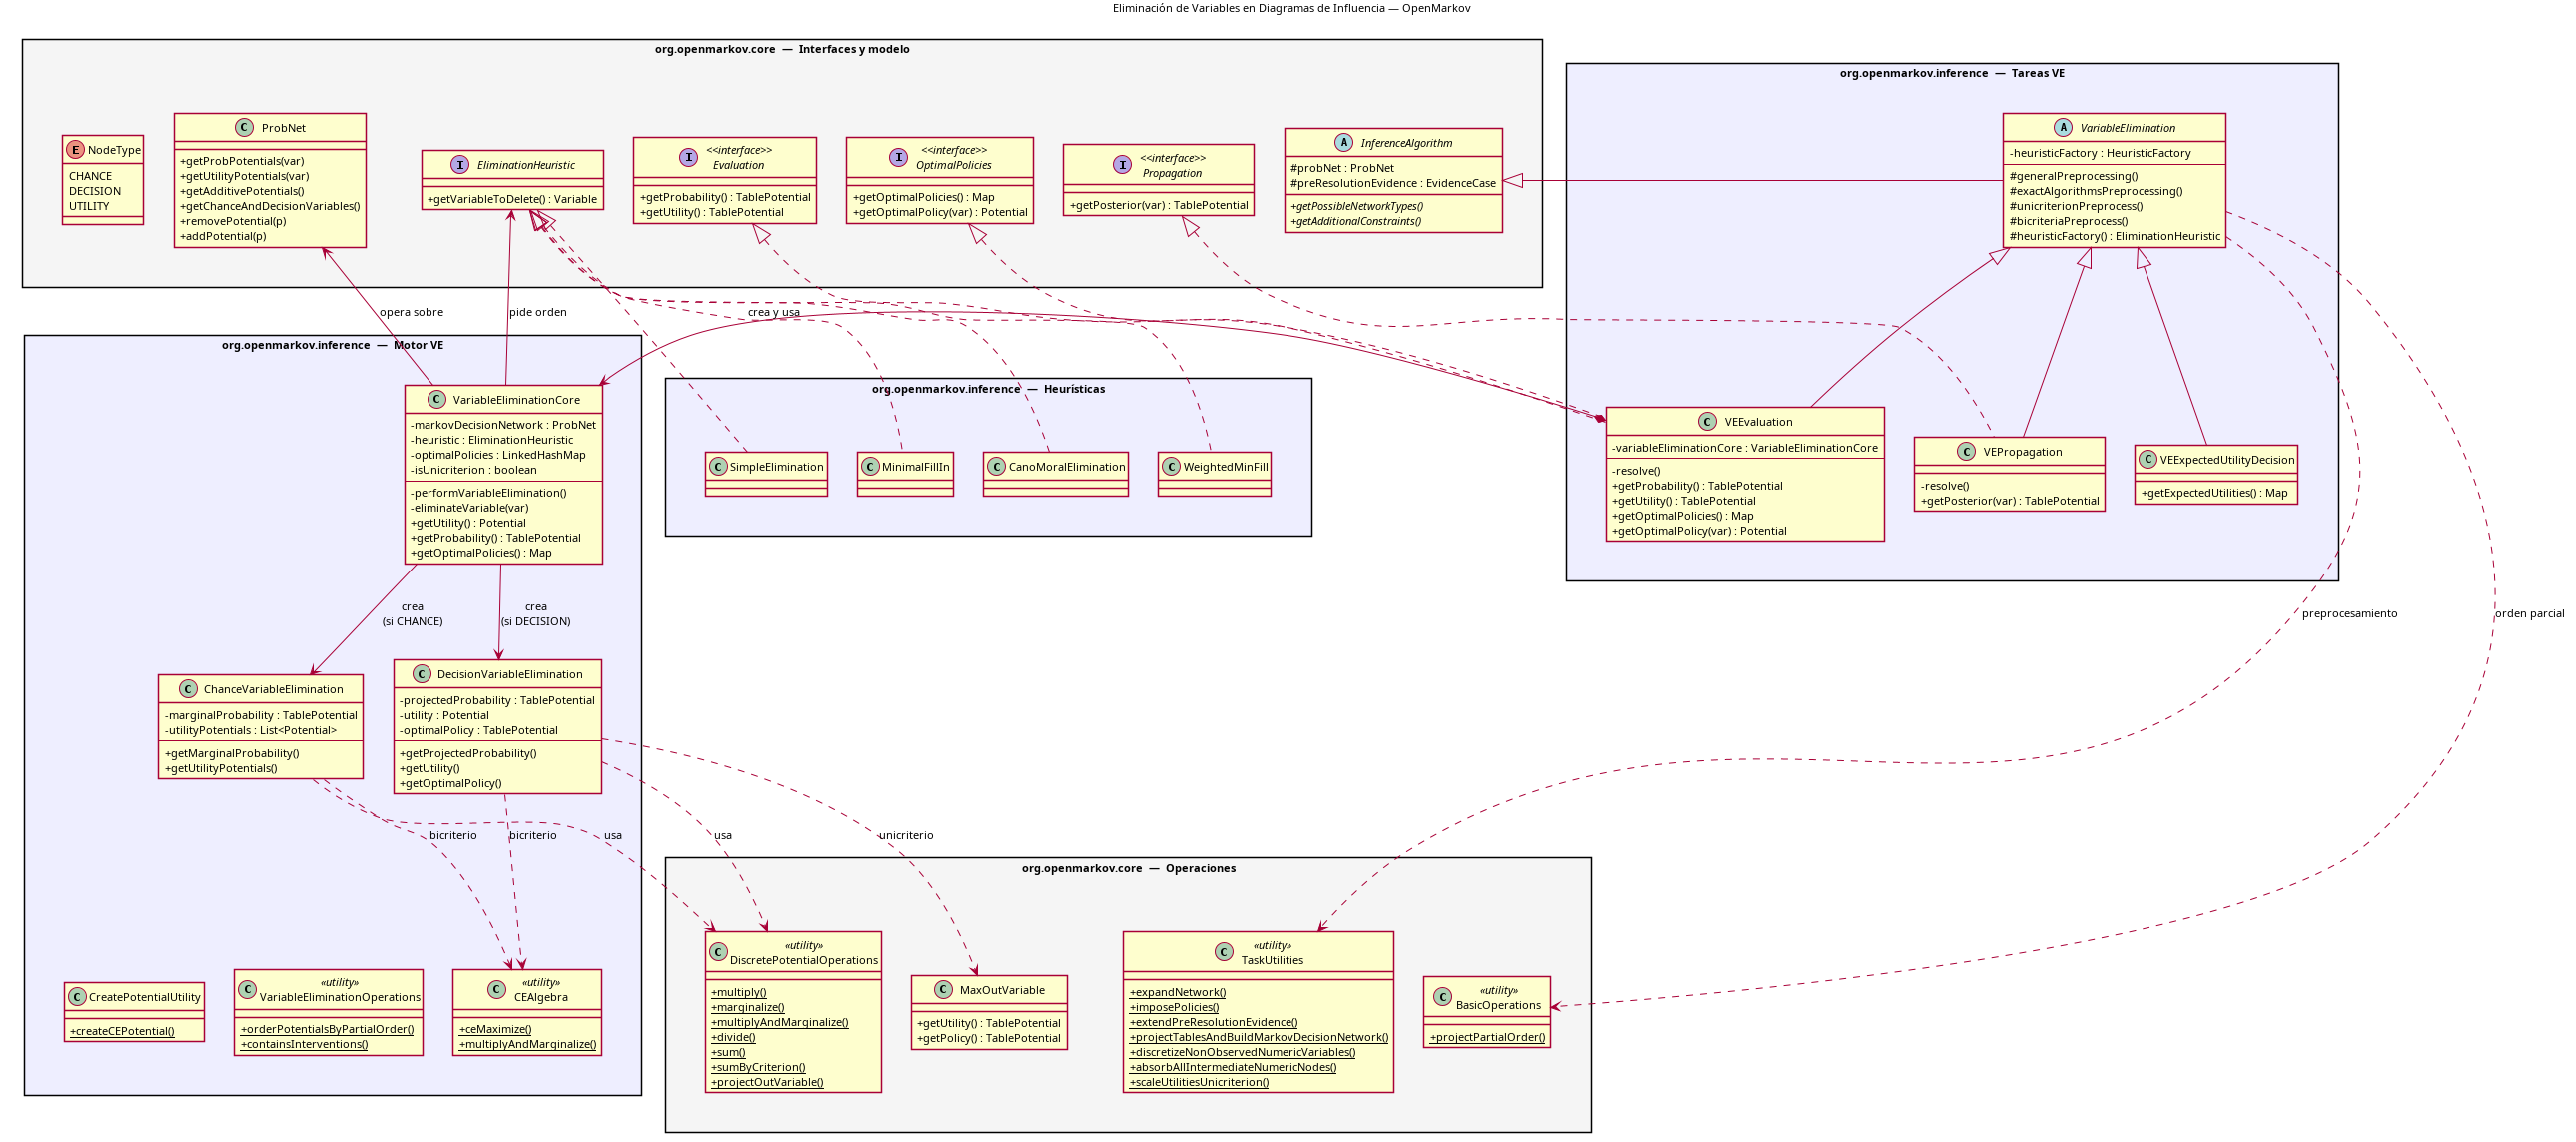
\includegraphics[width=\textwidth]{ve-influence-diagrams.png}
  \caption{Diagrama de clases de la eliminaci\'{o}n de variables para IDs.}
  \label{fig:class-diagram}
\end{figure}

\subsection{Diagrama de actividad}

Flujo de ejecuci\'{o}n con los dos caminos: marginalizaci\'{o}n (chance) y
maximizaci\'{o}n (decisi\'{o}n).

\begin{figure}[ht]
  \centering
  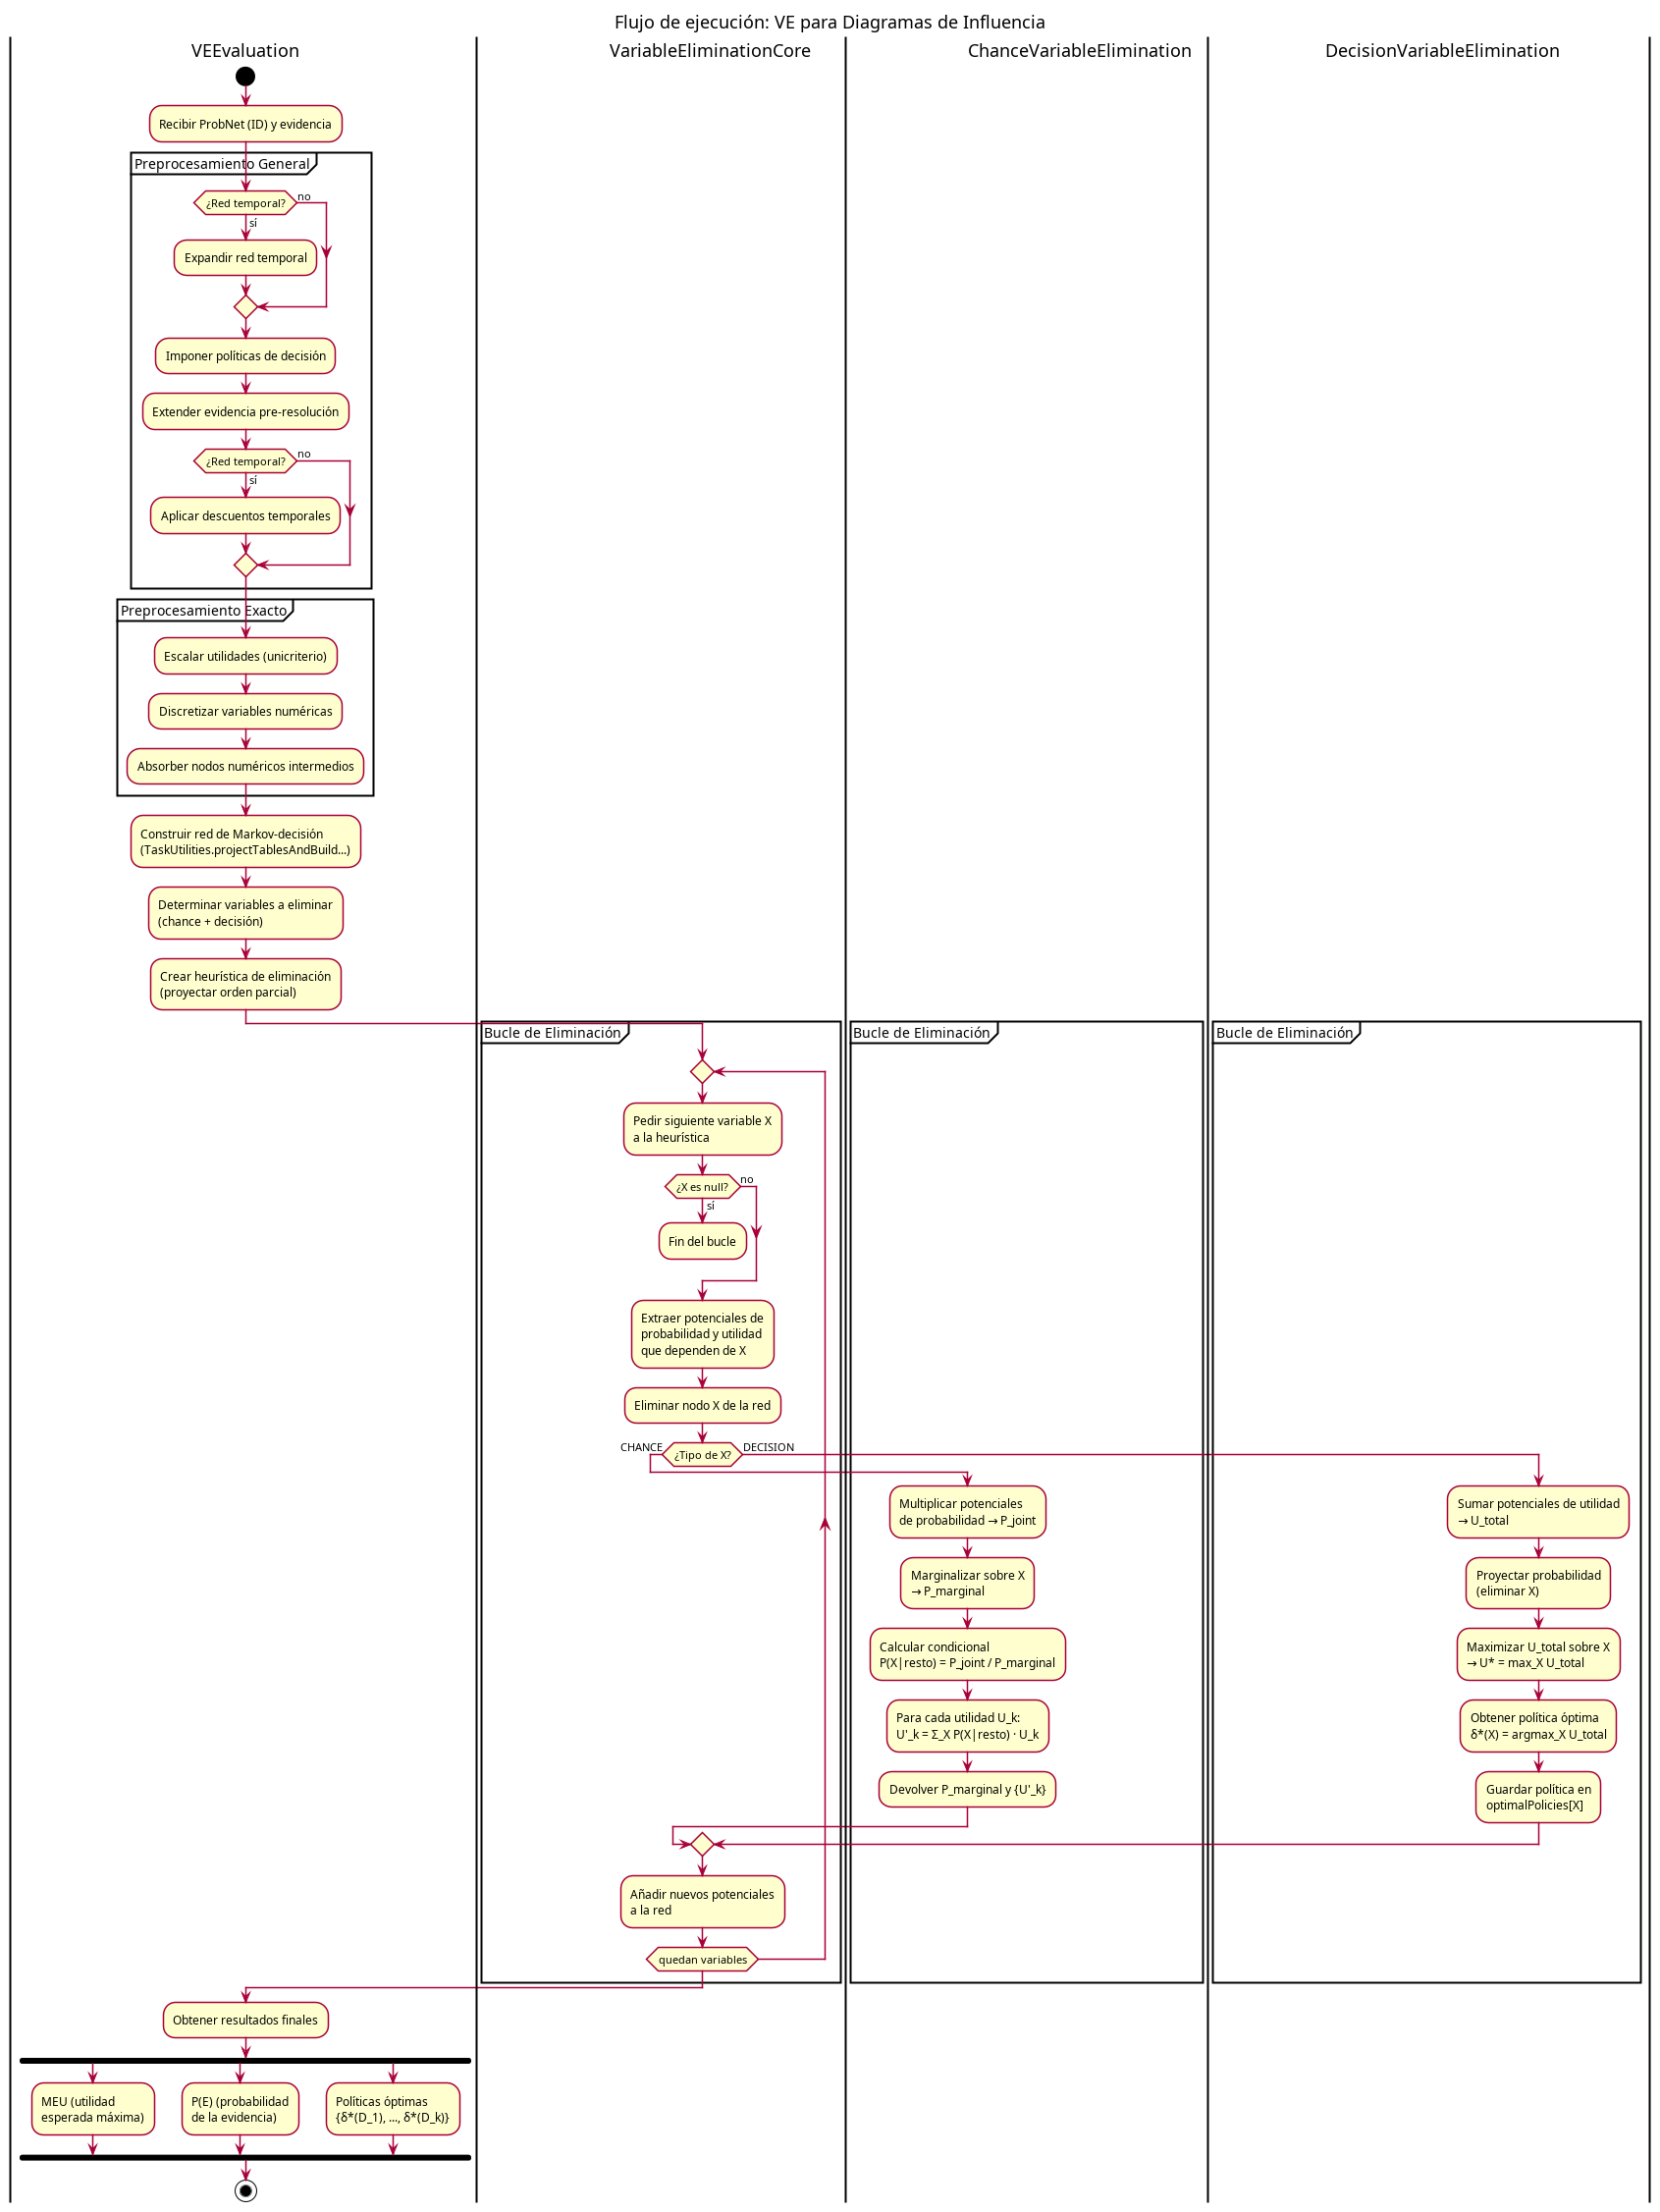
\includegraphics[width=0.75\textwidth]{ve-influence-diagrams-activity.png}
  \caption{Diagrama de actividad del algoritmo VE para IDs.}
  \label{fig:activity-diagram}
\end{figure}

\subsection{Diagrama de secuencia}

Interacci\'{o}n temporal entre los objetos principales durante la evaluaci\'{o}n.

\begin{figure}[ht]
  \centering
  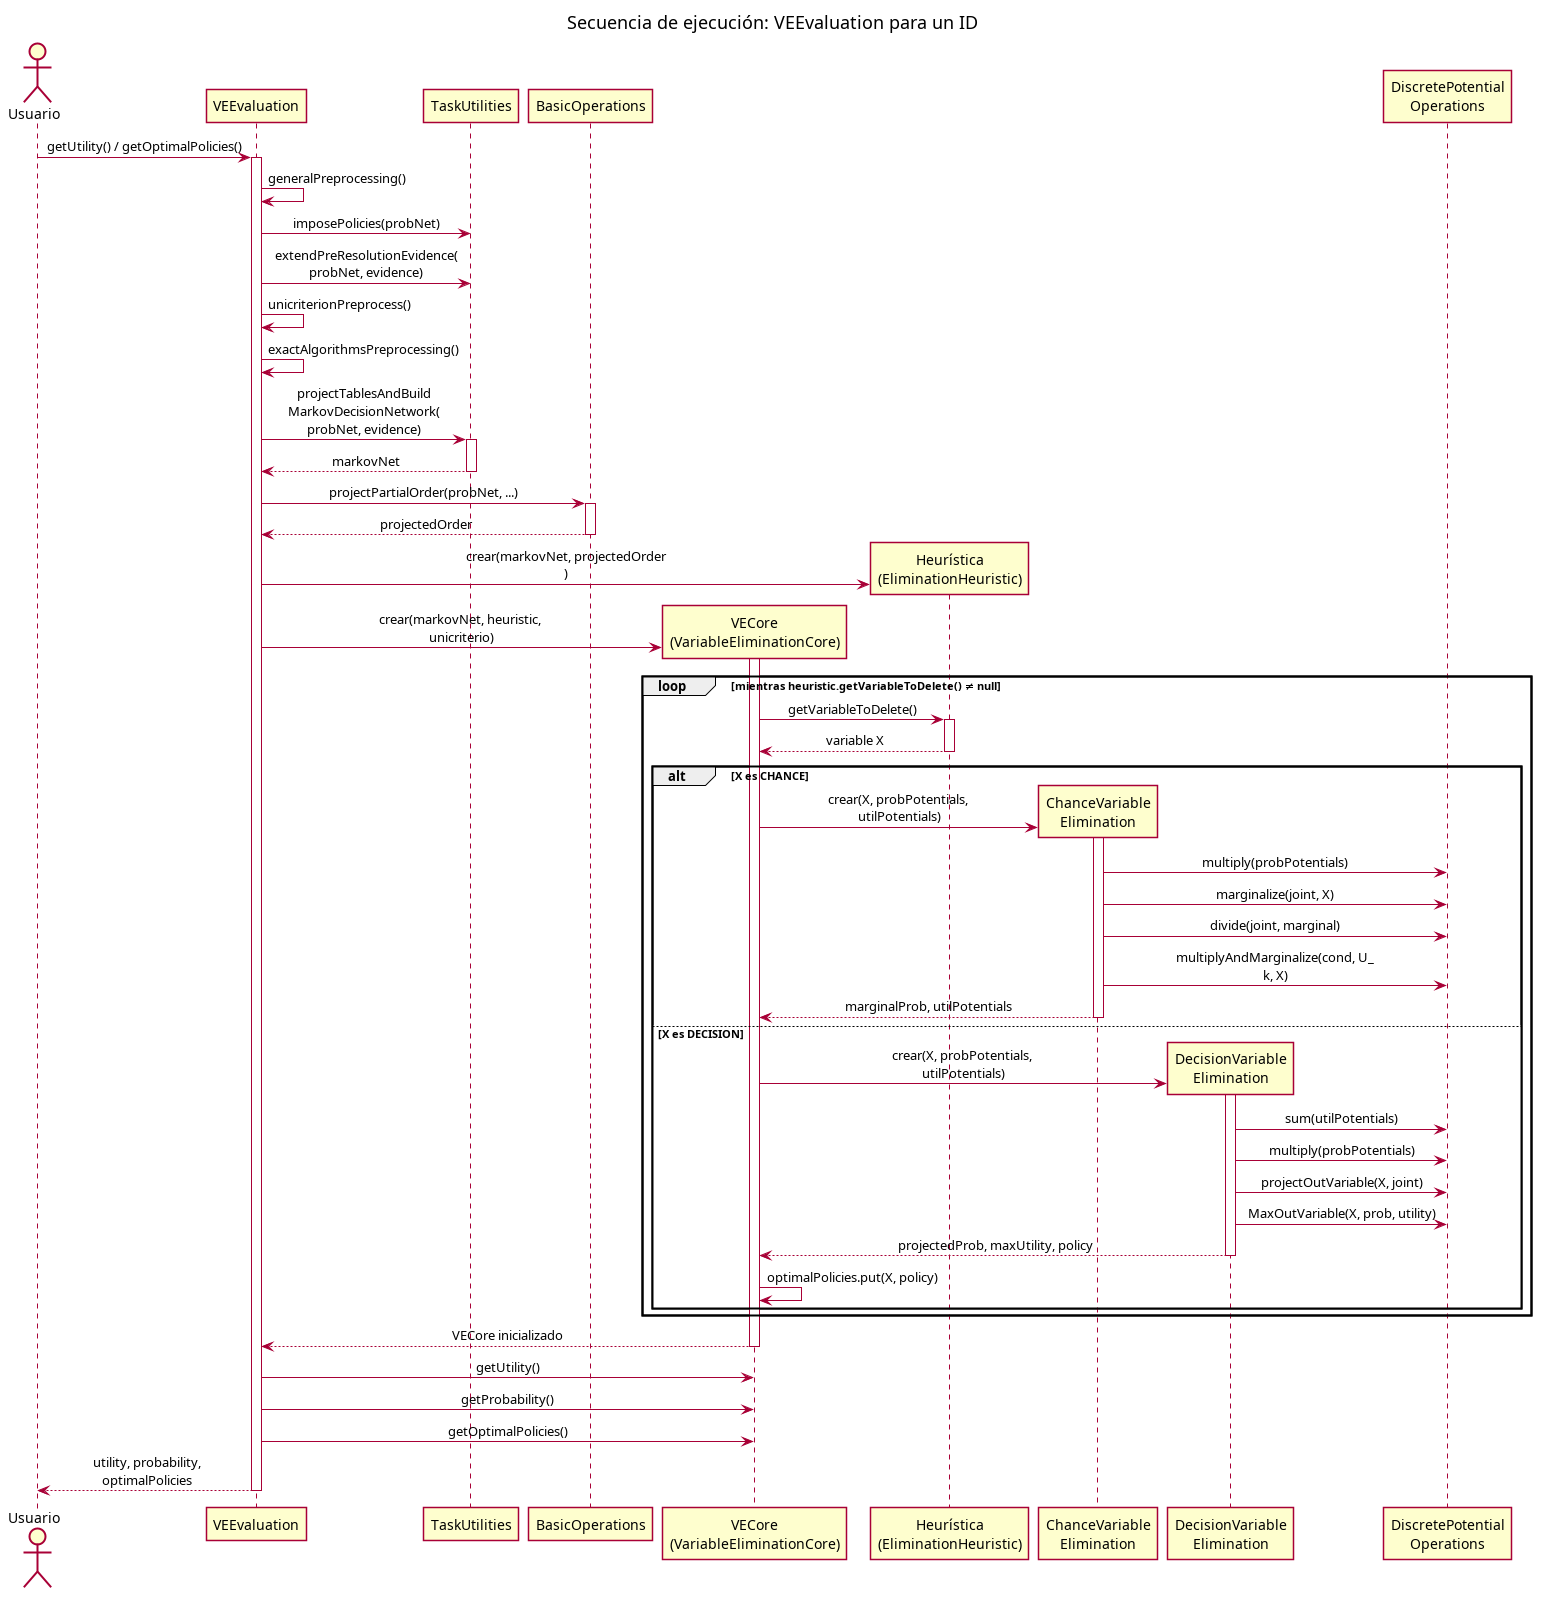
\includegraphics[width=\textwidth]{ve-influence-diagrams-sequence.png}
  \caption{Diagrama de secuencia de \texttt{VEEvaluation}.}
  \label{fig:sequence-diagram}
\end{figure}

\end{document}
